% The Diageo put: a short explainer (Simplified Technical English style)
% Build: tectonic report/explainer/diageo-put-explainer.tex
\documentclass[11pt,a4paper]{article}
\usepackage[margin=2.2cm]{geometry}
\usepackage[T1]{fontenc}
\usepackage{lmodern}
\usepackage{microtype}
\usepackage{xcolor}
\usepackage{booktabs}
\usepackage{enumitem}
\usepackage{tikz}
\usetikzlibrary{arrows.meta,positioning,calc}
\usepackage{pgfplots}
\pgfplotsset{compat=1.18}
\usepackage[hidelinks]{hyperref}

\definecolor{sblue}{HTML}{2A78D6}
\definecolor{sorange}{HTML}{EB6834}
\definecolor{sred}{HTML}{C0392B}
\definecolor{muted}{HTML}{5D5A52}
\definecolor{rule}{HTML}{DCD8CC}

\pgfplotsset{
  every axis/.append style={
    width=0.94\linewidth, height=5.2cm,
    axis lines*=left, ymajorgrids, grid style={rule},
    tick label style={font=\footnotesize, text=muted},
    label style={font=\footnotesize},
    legend style={font=\footnotesize, draw=none, fill=none, at={(0.5,1.03)}, anchor=south, legend columns=-1, /tikz/every even column/.append style={column sep=8pt}},
    legend cell align=left,
    /pgf/number format/1000 sep={,},
    enlarge x limits=0.12,
    scaled ticks=false,
    legend image code/.code={\draw[#1, draw=none] (0cm,-0.1cm) rectangle (0.25cm,0.12cm);},
  }
}

\newcommand{\src}[1]{\par\smallskip{\footnotesize\color{muted}Source: #1\par}}
\setlist[itemize]{leftmargin=1.4em, itemsep=2pt, topsep=4pt}
\setlength{\parindent}{0pt}
\setlength{\parskip}{6pt}

\begin{document}

{\footnotesize\color{muted}\MakeUppercase{LVMH \textperiodcentered{} IFRS \textperiodcentered{} FY2025 \textperiodcentered{} IAS 32.23}}\par
{\LARGE\bfseries The Diageo put: a \texteuro6.3bn debt that LVMH does not call debt\par}
\medskip
Diageo owns 34\% of Mo\"et Hennessy (MH). Diageo can force LVMH to buy this stake at any time. LVMH records this obligation as a liability. The accounting method keeps large value changes out of the income statement.

\medskip
\begin{center}
\begin{tabular}{@{}cccc@{}}
\toprule
\textbf{\Large \texteuro6.3bn} & \textbf{\Large 92\%} & \textbf{\Large $-$\texteuro30bn} & \textbf{\Large \texteuro0} \\
\footnotesize Put liability, & \footnotesize Of reported net debt. & \footnotesize Fall in LVMH's value & \footnotesize Of that fall in the \\
\footnotesize 31 Dec 2025 & \footnotesize LVMH excludes it. & \footnotesize of MH, 2021--2025 & \footnotesize income statement \\
\bottomrule
\end{tabular}
\end{center}

\section*{1. What is the issue?}
A 1994 contract gives Diageo a put option. Diageo can sell its 34\% to LVMH with six months' notice. The price is 80\% of the fair value of MH on that date. IAS~32.23 says: record this as a financial liability. IFRS does not say where the other side of the entry goes.

LVMH uses an old French method (note 1.13). It removes Diageo's minority interest. It puts the difference into goodwill. Each year, the change in the put value also goes to goodwill. It does not go to profit or loss.

\begin{center}
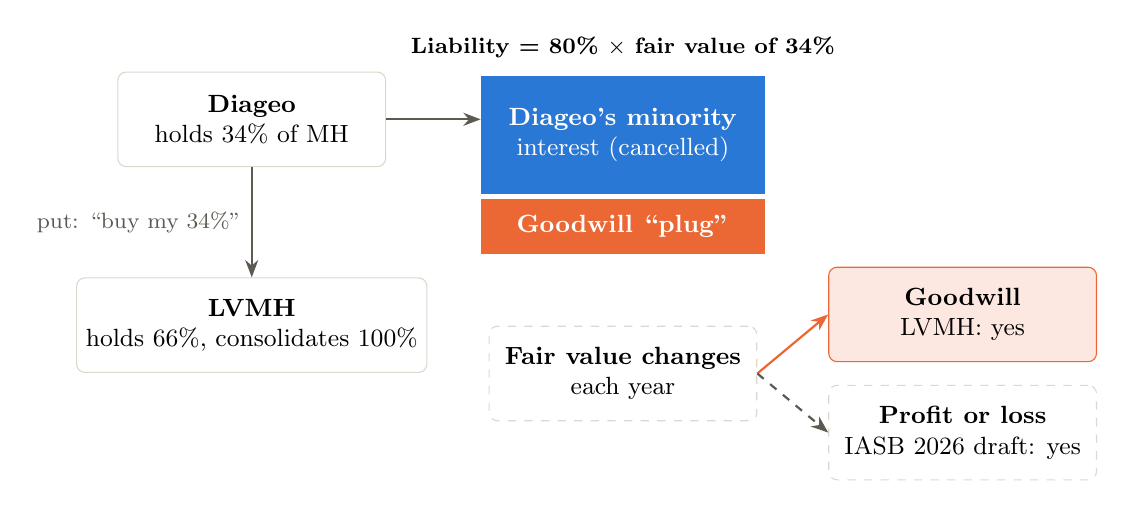
\begin{tikzpicture}[
  font=\small,
  box/.style={draw=rule, rounded corners=3pt, align=center, minimum width=3.4cm, minimum height=1.2cm},
  arr/.style={-{Stealth[length=2.2mm]}, thick, muted}]
  \node[box] (diageo) {\textbf{Diageo}\\holds 34\% of MH};
  \node[box, below=1.4cm of diageo] (lvmh) {\textbf{LVMH}\\holds 66\%, consolidates 100\%};
  \draw[arr] (diageo) -- node[left, font=\footnotesize]{put: ``buy my 34\%''} (lvmh);

  \node[fill=sblue, text=white, minimum width=3.6cm, minimum height=1.5cm, align=center, right=1.2cm of diageo, yshift=-0.2cm] (nci) {\textbf{Diageo's minority}\\interest (cancelled)};
  \node[fill=sorange, text=white, minimum width=3.6cm, minimum height=0.7cm, below=0.05cm of nci, align=center] (gw) {\textbf{Goodwill ``plug''}};
  \node[above=0.1cm of nci, font=\footnotesize\bfseries] {Liability = 80\% $\times$ fair value of 34\%};
  \draw[arr] (diageo.east) -- (nci.west |- diageo.east);

  \node[box, dashed, below=0.9cm of gw] (fv) {\textbf{Fair value changes}\\each year};
  \node[box, fill=sorange!15, draw=sorange, right=0.9cm of fv, yshift=0.75cm] (g2) {\textbf{Goodwill}\\LVMH: yes};
  \node[box, dashed, right=0.9cm of fv, yshift=-0.75cm] (pl) {\textbf{Profit or loss}\\IASB 2026 draft: yes};
  \draw[arr, sorange] (fv.east) -- (g2.west);
  \draw[arr, dashed] (fv.east) -- (pl.west);
\end{tikzpicture}
\src{LVMH FY2025 Financial Documents (FD), note 1.13 (p.~33) and note 21 (p.~56); IASB FICE tentative decision, 22 Sep 2026.}
\end{center}

\section*{2. Size}
The goodwill plug fell from \texteuro9.1bn to \texteuro0.4bn. The blue part is Diageo's share of MH book equity. It stays at about \texteuro4.3bn. The orange part is the goodwill plug. It shows the value above book. This part almost disappeared.

\begin{center}
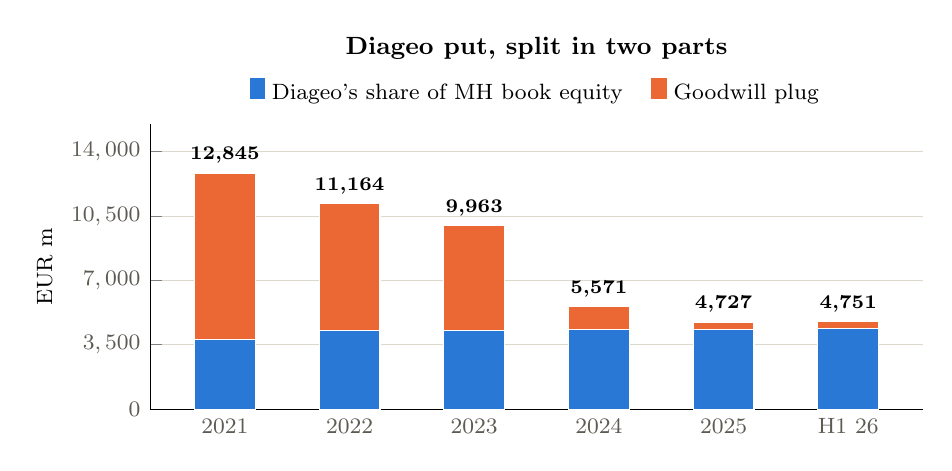
\begin{tikzpicture}
\begin{axis}[
  ybar stacked, bar width=22pt, ymin=0, ymax=15500,
  ytick={0,3500,7000,10500,14000},
  symbolic x coords={2021,2022,2023,2024,2025,H1 26}, xtick=data,
  ylabel={EUR m},
  title={\small\bfseries Diageo put, split in two parts},
  title style={yshift=14pt},
]
\addplot[fill=sblue, draw=white] coordinates {(2021,3775) (2022,4265) (2023,4281) (2024,4332) (2025,4341) (H1 26,4369)};
\addplot[fill=sorange, draw=white]
  coordinates {(2021,9070) (2022,6899) (2023,5682) (2024,1239) (2025,386) (H1 26,382)};
\foreach \x/\v/\t in {2021/12845/12{,}845, 2022/11164/11{,}164, 2023/9963/9{,}963, 2024/5571/5{,}571, 2025/4727/4{,}727, H1 26/4751/4{,}751}
  {\edef\tmp{\noexpand\node[font=\noexpand\scriptsize\noexpand\bfseries, anchor=south] at (axis cs:\x,\v) {\t};}\tmp}
\legend{Diageo's share of MH book equity, Goodwill plug}
\end{axis}
\end{tikzpicture}
\src{LVMH FD FY2021--25, note 4 (goodwill) and note 18 (minority interests); H1-2026 half-year report, notes 4 and 18. Labels show the total.}
\end{center}

\begin{center}
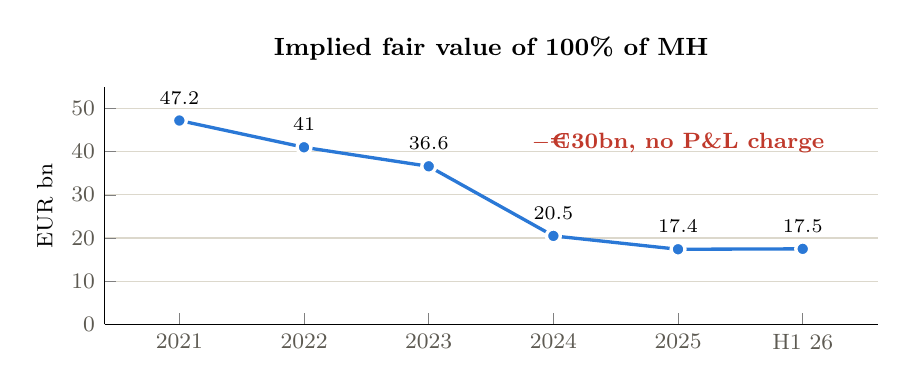
\begin{tikzpicture}
\begin{axis}[
  height=4.6cm, ymin=0, ymax=55, ytick={0,10,...,50},
  symbolic x coords={2021,2022,2023,2024,2025,H1 26}, xtick=data,
  ylabel={EUR bn},
  title={\small\bfseries Implied fair value of 100\% of MH},
]
\addplot[sblue, very thick, mark=*, mark size=2.5pt, mark options={fill=sblue, draw=white},
  nodes near coords, every node near coord/.append style={font=\scriptsize\bfseries, anchor=south, yshift=2pt, text=black}]
  coordinates {(2021,47.2) (2022,41.0) (2023,36.6) (2024,20.5) (2025,17.4) (H1 26,17.5)};
\node[font=\footnotesize\bfseries, text=sred] at (axis cs:2025,42) {$-$\texteuro30bn, no P\&L charge};
\end{axis}
\end{tikzpicture}
\src{Calculation: (goodwill plug + Diageo's equity share) $\div$ 0.8 $\div$ 0.34. Accuracy is about $\pm$10\%, because the plug also includes small non-Diageo puts.}
\end{center}

The cause is real. Cognac demand fell in the US and China. Wines \& Spirits profit from recurring operations fell from \texteuro2.1bn (2023) to \texteuro1.0bn (2025).

\section*{3. Materiality}
The put almost doubles net debt. LVMH does not include the put in net financial debt (note 19.1). But Diageo can demand cash in six months. A buyer must treat it as debt.

\begin{center}
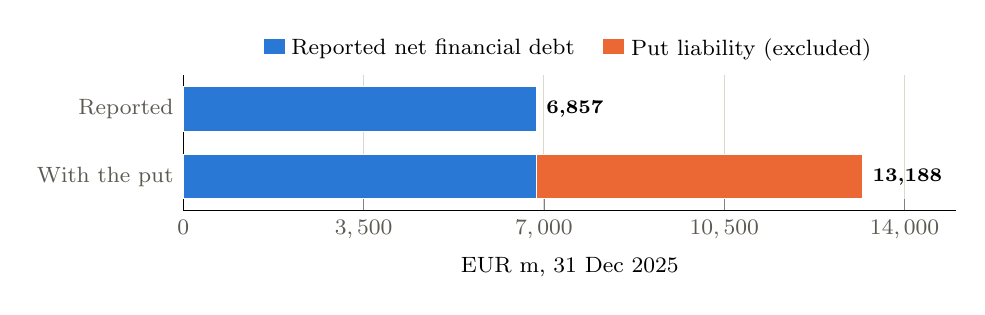
\begin{tikzpicture}
\begin{axis}[
  xbar stacked, height=3.3cm, bar width=16pt,
  xmin=0, xmax=15000, xtick={0,3500,7000,10500,14000},
  symbolic y coords={With the put,Reported}, ytick=data,
  axis lines*=left, ymajorgrids=false, xmajorgrids, enlarge y limits=0.5, enlarge x limits=false,
  xlabel={EUR m, 31 Dec 2025},
]
\addplot[fill=sblue, draw=white] coordinates {(6857,Reported) (6857,With the put)};
\addplot[fill=sorange, draw=white] coordinates {(0,Reported) (6331,With the put)};
\node[font=\scriptsize\bfseries, anchor=west] at (axis cs:6857,Reported) {6,857};
\node[font=\scriptsize\bfseries, anchor=west] at (axis cs:13188,With the put) {13,188};
\legend{Reported net financial debt, Put liability (excluded)}
\end{axis}
\end{tikzpicture}
\src{LVMH FY2025 FD, balance sheet (p.~26) and note 19.1 (p.~53).}
\end{center}

\section*{4. Impact on profit}
In September 2026 the IASB decided (tentatively) that put remeasurement must go to profit or loss. If this rule applied before, group net profit would move by up to 35\%.

\begin{center}
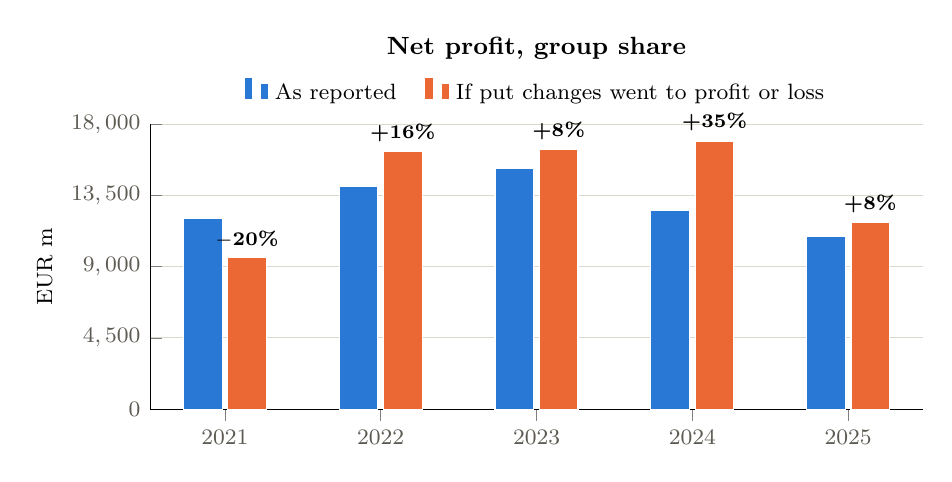
\begin{tikzpicture}
\begin{axis}[
  ybar, bar width=14pt, ymin=0, ymax=18000, ytick={0,4500,9000,13500,18000},
  symbolic x coords={2021,2022,2023,2024,2025}, xtick=data,
  ylabel={EUR m},
  title={\small\bfseries Net profit, group share},
  title style={yshift=14pt},
]
\addplot[fill=sblue, draw=white] coordinates {(2021,12036) (2022,14084) (2023,15174) (2024,12550) (2025,10878)};
\addplot[fill=sorange, draw=white,
  nodes near coords, point meta=explicit symbolic,
  every node near coord/.append style={font=\scriptsize\bfseries, anchor=south}]
  coordinates {(2021,9569)[$-$20\%] (2022,16288)[+16\%] (2023,16409)[+8\%] (2024,16928)[+35\%] (2025,11778)[+8\%]};
\legend{As reported, If put changes went to profit or loss}
\end{axis}
\end{tikzpicture}
\src{LVMH income statements (FY2023 FD p.~24; FY2025 FD p.~24). Adjustment = ``changes in purchase commitments'' in note 4, with the opposite sign. Pre-tax, illustrative.}
\end{center}

\begin{center}
\small
\begin{tabular}{@{}lrrrrr@{}}
\toprule
EUR m & 2021 & 2022 & 2023 & 2024 & 2025 \\
\midrule
As reported & 12,036 & 14,084 & 15,174 & 12,550 & 10,878 \\
Put remeasurement & $-$2,467 & +2,204 & +1,235 & +4,378 & +900 \\
If via P\&L & 9,569 & 16,288 & 16,409 & 16,928 & 11,778 \\
Change & $-$20\% & +16\% & +8\% & +35\% & +8\% \\
\bottomrule
\end{tabular}
\end{center}

\section*{5. Why the number is uncertain}
The value is a management estimate.
\begin{itemize}
  \item \textbf{Method change.} Until H1 2025, LVMH used market multiples. In FY2025 it changed to a DCF. LVMH gives no reason.
  \item \textbf{No sensitivity.} LVMH gives no sensitivity for the put or for Wines \& Spirits.
  \item \textbf{Two parties, two values.} LVMH's basis gives about \texteuro17bn for 100\% of MH. Diageo's multiples give about \texteuro13bn.
  \item \textbf{Price at a low point.} At the 2023 value, the same 34\% was worth about \texteuro12.5bn. Now it is about \texteuro5.9bn.
\end{itemize}

\section*{6. What should we do?}
\textbf{Do not stop the deal for this issue. Change the price.}
\begin{itemize}
  \item Add the put (\texteuro6.3bn) to net debt in the valuation.
  \item Use \texteuro5--6bn as the minimum cost to own 100\% of MH.
  \item Get the full 1994 agreement. Check the change-of-control terms.
  \item Value Wines \& Spirits with our own model. Do not use LVMH's goodwill numbers.
  \item Remove the put remeasurement from covenants and earn-outs. The IASB rule can change profit by billions.
\end{itemize}

\end{document}
